\section{Introduzione}
L'accelerazione del progresso tecnologico, la progressiva liberalizzazione degli scambi commerciali e il grande sviluppo delle comunicazioni hanno portato alla nascita del mercato globale. Le aziende realizzano nuovi prodotti a ritmi sempre più elevati con prezzi sempre più competitivi ed economici; questo spinge i consumatori a credere che gli oggetti in loro possesso diventino obsoleti nell'arco di pochi mesi e li invita quindi ad acquistare sempre di più. Questo continuo ciclo d'acquisto è alla base del consumismo moderno che negli ultimi anni sta producendo sempre più spazzatura mettendo in pericolo il pianeta intero. Numerosi studi \cite{Sprechi} rivelano che il problema spesso risiede nel fatto che i consumatori e le aziende, non sapendo che fare dei prodotti obsoleti, li buttano via anche se funzionanti. 
\medskip

Rius.Co. cerca di risolvere questa problematica attraverso una piattaforma per il riuso online che permette a chiunque di poter acquisire oggetti di seconda mano funzionanti in modo del tutto gratuito e facilmente accessibile. Rius.Co. si ispira ai già esistenti centri del riuso presenti nella Regione Marche, ma innova portando questa iniziativa solidale nelle mani di tutti attraverso il sito web sulla quale si appoggerà la piattaforma. Il sito web consiste in un e-commerce customer-to-customer in cui tutti possono offrire e richiedere oggetti usando la moneta di scambio virtuale coniata a questo scopo: il Green Coin. Spendendo un Green Coin gli utenti potranno richiedere ed ottenere un prodotto da un altro utente appartenente alla piattaforma. Ogni prodotto, qualsiasi esso sia, se funzionante e in buone condizioni potrà essere inserito nel Marketplace dove gli verrà assegnato il “prezzo” di un Green Coin a prescindere dal suo valore economico che è trascurato in quanto si tratta di oggetti che altrimenti sarebbero stati buttati in discarica. 
\medskip

\begin{figure}[hb]
    \subfigure[Logo Rius.Co.]{
\includegraphics[scale=.12]{images/logo.png}}
    \hfill
    \subfigure[Logo esteso Rius.Co.]{
\includegraphics[scale=.06]{images/riusco.png}}
    \hfill
    \subfigure[Green Coin]{
\includegraphics[scale=.07]{images/green_coin.png}}
    \caption{Loghi ed icone dell'azienda}
\end{figure}
\clearpage

Un importante punto di forza della piattaforma è la possibilità d'integrazione con i già esistenti centri del riuso locali facilitandone il flusso degli oggetti e aiutandoli quindi a costruire un inventario completo o ad alleviare la mole di lavoro e la quantità di oggetti che questi centri, spesso di modeste dimensioni, gestiscono con difficoltà. I centri del riuso locali possono quindi beneficiare in modo considerevole da una collaborazione con la piattaforma Rius.Co. che ne guadagnerebbe l'opportunità di ingrandire il proprio bacino d'utenza. 
La piattaforma può anche servire come rete di collegamento dei centri del riuso già esistenti, aiutandoli nella comunicazione e negli scambi di oggetti in modo efficiente. Il progetto risulta quindi semplice dal punto di vista operativo, economico dal punto di vista finanziario e sostenibile dal punto di vista ambientale. 
\medskip

Rius.Co. ha in comune numerosi obiettivi con l'importante Agenda 2030, un programma d'azione per le persone, il pianeta e la prosperità sottoscritto nel 2015 dai Paesi membri dell'ONU \cite{Agenda2030}, questi obiettivi sono: 
\begin{itemize}
    \item 1° Obiettivo – “Porre fine alla povertà in tutte le sue forme”: chiunque può commerciare gratuitamente sulla piattaforma a prescindere dal proprio reddito o situazione economica; 
    \item 11° Obiettivo – “Rendere le città e gli insediamenti umani inclusivi, sicuri, duraturi e sostenibili”: le città possono diventare più sostenibili e sicure grazie alla riduzione dei rifiuti; 
    \item 12° Obiettivo – “Garantire modelli sostenibili di produzione e di consumo”: la piattaforma offre un modello sostenibile di consumo congruo alla vita d'oggi; 
    \item 13° Obiettivo – “Promuovere azioni, a tutti i livelli, per combattere il cambiamento climatico”: promuovendo il riutilizzo degli oggetti e, di conseguenza, scoraggiando l'accumulo di rifiuti nelle discariche, Rius.co. supporta la lotta contro il cambiamento climatico. 
\end{itemize}
\begin{figure}[hb]
    \centering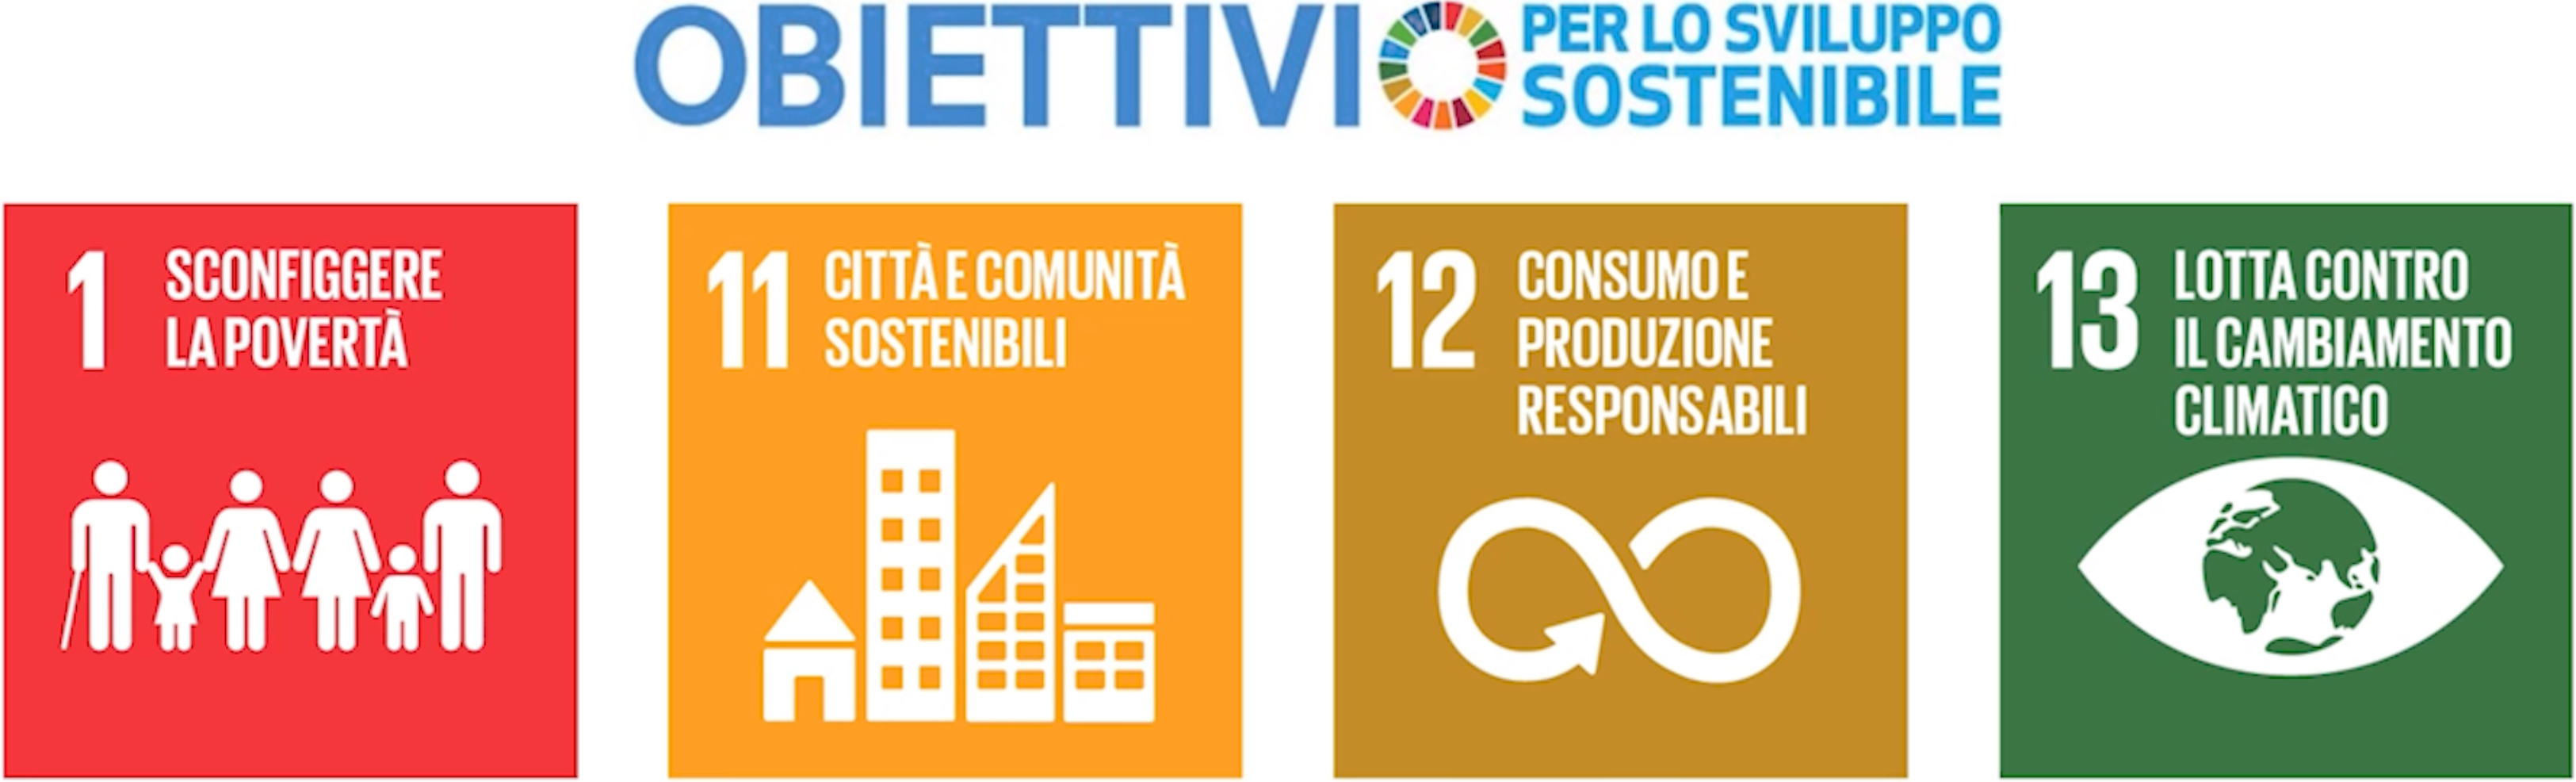
\includegraphics[scale=0.1]{images/agenda_2030.png}
    \caption{Obiettivi 1, 11, 12 e 13 dell'Agenda 2030}
\end{figure}
\clearpage
